\documentclass[a4paper,11 pt,oneside]{book}
\linespread{1.5}
\usepackage[left=2.5cm, right=2.5cm, top=2.5cm, bottom=2.5cm]{geometry}
\usepackage[utf8]{inputenc}	%Qui ho cambiato da italian a utf8
\usepackage[italian]{babel}
\usepackage{amsfonts}
\usepackage{amsmath}
\usepackage{amsthm}
\usepackage{amssymb,amsmath,color}
\usepackage{cite}
\usepackage{graphicx}
\usepackage[utf8]{inputenc}
\usepackage{subfigure}
\usepackage{inputenc}
\usepackage{float}
\usepackage{algorithm}
\usepackage{algpseudocode}
\usepackage{algorithmicx}
\usepackage{pdfpages}
\usepackage{systeme}
\theoremstyle{definition}
\newtheorem{definition}{Definition}[section]
%\theoremstyle{theorem}
%\newtheorem{theorem}{Theorem}[section]
%\theoremstyle{lemma}
%\newtheorem{lemma}{Lemma}[section]

\usepackage{fancyhdr}
\pagestyle{fancy}
\fancyhf{}
\fancyhead[L]{\leftmark}
\fancyfoot[C]{\thepage}

\tolerance=1
\emergencystretch=\maxdimen
\hyphenpenalty=10000
\hbadness=10000


%I miei import
\usepackage{underscore}
\setlength\parindent{0pt}

\usepackage{seqsplit}
\usepackage{tcolorbox}
\usepackage{listings}

\usepackage{color}

\graphicspath{{./figs/}}

\usepackage{hyperref}
\hypersetup{
     colorlinks=true,
     linkcolor=black,
     urlcolor=blue,
}

\usepackage{listings}
\definecolor{mygray}{gray}{0.95}
\lstset{ 
language=C++, 
basicstyle=\ttfamily\footnotesize,
showspaces=false,
showstringspaces=false,
columns=flexible,
breaklines=true,
breakatwhitespace=true,
tabsize=4,
backgroundcolor=\color{mygray},
numbersep=5pt,
xleftmargin=.22in,
xrightmargin=.22in
}

\newtcolorbox{redbox}[1]{
colback=red!5!white,
colframe=red!75,
fonttitle=\bfseries,
title=#1,
}

\definecolor{lightgray}{gray}{0.95}

\lstset{
basicstyle=\ttfamily\footnotesize,
showspaces=false,
showstringspaces=false,
columns=flexible,
breaklines=true,
breakatwhitespace=true,
tabsize=4,
backgroundcolor=\color{lightgray},
numbersep=5pt
}

\begin{document}


	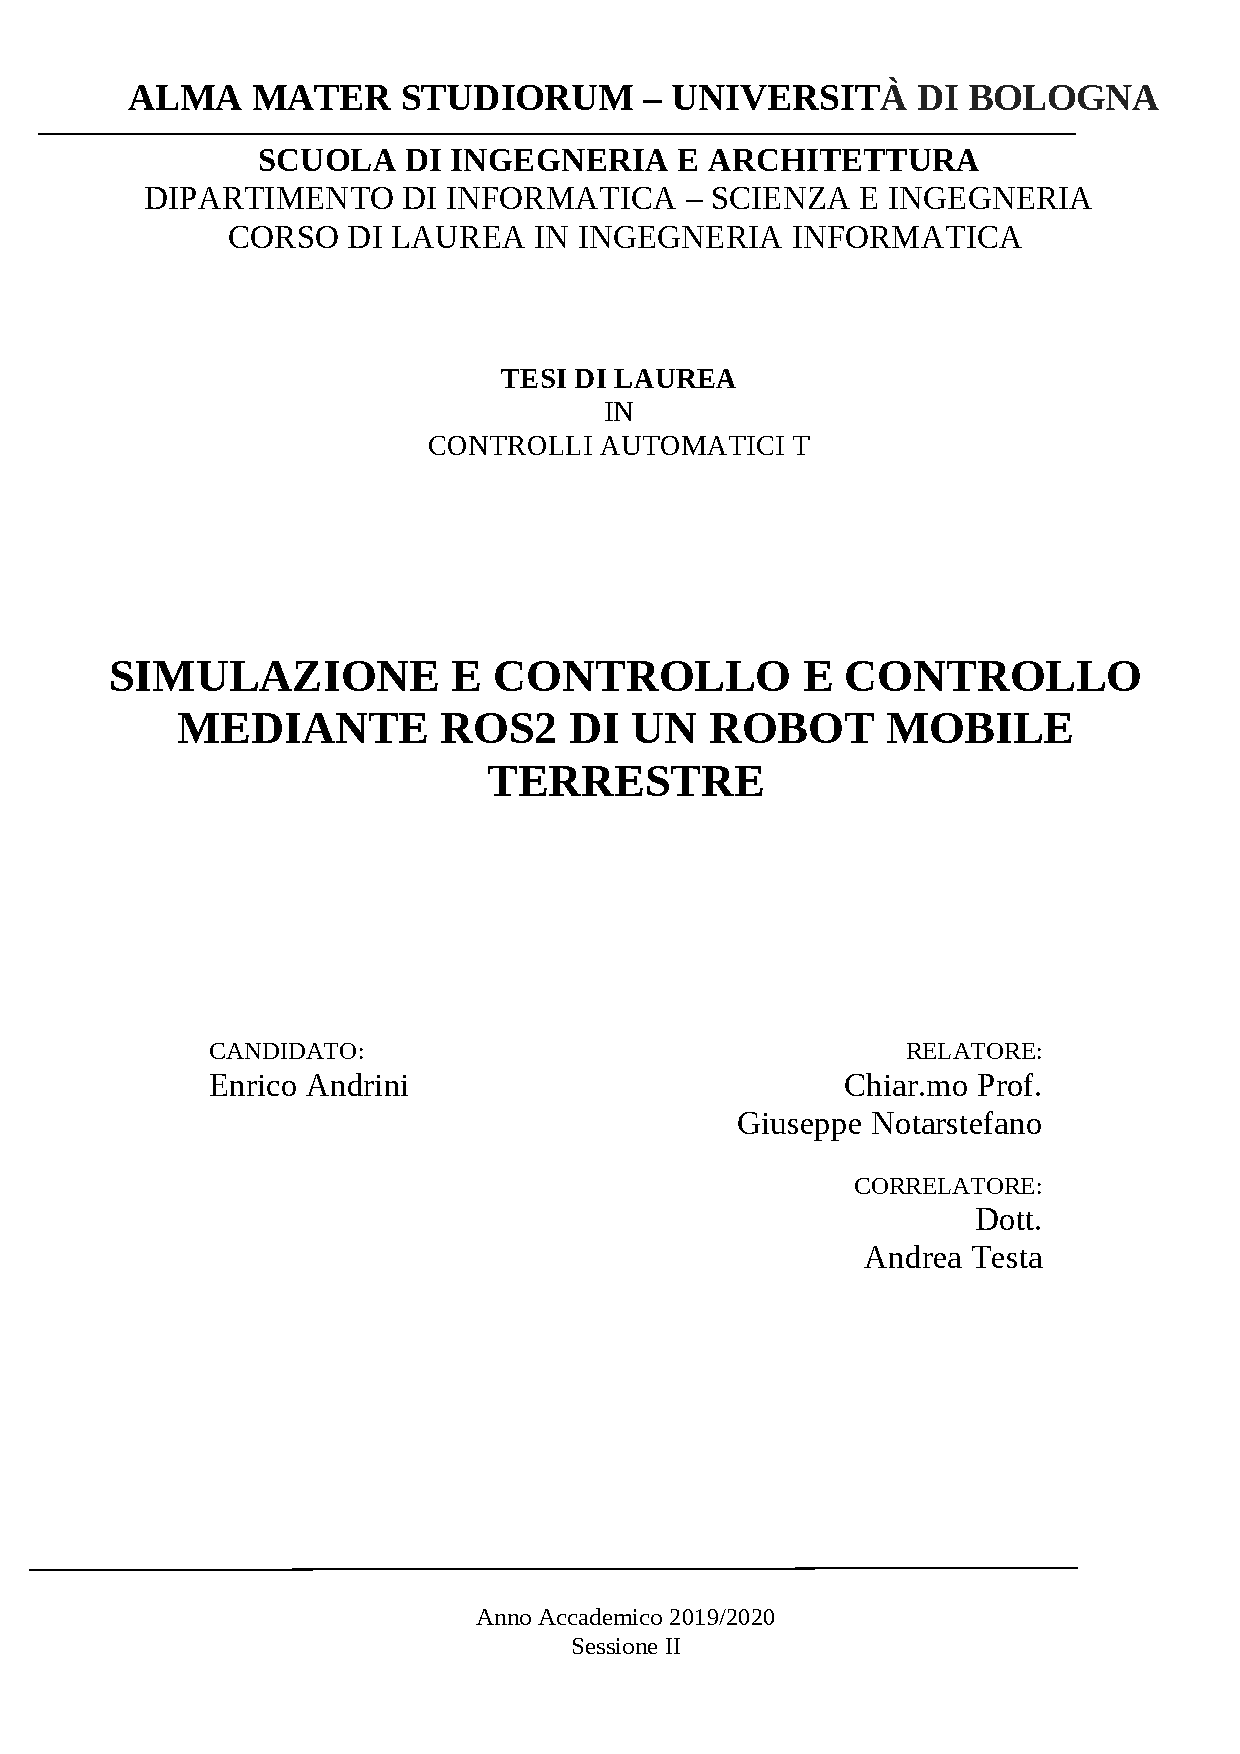
\includepdf{figs/Frontespizio.pdf} 
	\newpage
	\thispagestyle{empty}

	%%%%%% ABSTRACT %%%%%%%%%%
\chapter*{Abstract}
Progettare software attraverso architetture modulari è fondamentale per garantire semplicità e successive estensioni. Per questo nel seguente elaborato è proposta un'architettura modulare, basata sul framework ROS 2 e sull'ambiente di simulazione Gazebo, per il controllo e la simulazione di un robot mobile terrestre. In particolare, sono analizzati i componenti fondamentali di ROS 2 e Gazebo, necessari per sviluppare un'architettura per il controllo di robot. 
Viene poi introdotto il modello matematico dell'uniciclo, che permette di catturare le proprietà fondamentali di un robot mobile terrestre pur mantendendo un elevato livello di astrazione. Invece che cercare unicamente di portare nel minor tempo possibile il robot nella posizione verrà valorizzata la qualità del percorso cercando delle traiettorie efficienti e stabili.
In seguito sarà sviluppata l'architettura tramite ROS 2.
Essa è composta da due unità fondamentali di cui una si occupa della pianificazione e la seconda di implementare la legge di controllo.
Come dice lo stesso nome, il pianificatore si occupa di scegliere un punto nello spazio e l'assetto finale del robot mentre il controllore risolve il cosidetto \emph{parking problem} in quanto permette il posizionamento del robot nell'intorno di un punto con un preciso orientamento nello spazio. Infatti garantirà il raggiungimento della posizione prestabilita modificando la velocità angolare rispetto all'asse \emph{z} del robot in funzione dei risultati ottenuti dalla legge di controllo. Inoltre per garantire stabilità durante la fase di arrivo, il robot decellererà maggiormente all'avvicinamento dell'obiettivo.
La divisione in moduli che hanno compiti separati ma che rimangono comunque strettamente connessi è il punto di forza dell'applicazione.
Inoltre è stato utilizzato Gazebo per eseguire numerosi test che provassero la concretezza ed affidabilità dell'architettura implementata. 

%%%%%%%%%%%%%%%%%%%%%%%%%%%

	\tableofcontents\thispagestyle{empty}
	\listoffigures\thispagestyle{empty}
	\mainmatter
	%%%%%% INTRODUZIONE %%%%%%%%%%
	\chapter*{Introduzione}
	\addcontentsline{toc}{chapter}{Introduzione}
	

\section*{Motivazione}
Sin dall'avvento dei primi calcolatori moderni il concetto di robot come macchina artificiale in grado di svolgere compiti assegnatigli dall'uomo, per supervisione diretta o tramite il perseguimento di regole precise specificate a priori, è da molto oggetto di ricerche e di studi che hanno portato a solide basi sulle quali poter implementare sistemi particolarmente evoluti con capacità articolate.
La rapida evoluzione dei microprocessori ed il conseguente aumento della potenza di calcolo ha reso possibile la concretizzazione di un un'idea già nota alla società e già teorizzata nella letteratura ingegneristica.
Per garantire la progettazione di robot efficienti e per poter concretizzarli entrano in gioco materie fondamentali come l'analisi matematica per la realizzazione di modelli o la fisica che ne permette la messa in pratica nel mondo reale. L'informatica,  invece, è la componente fondamentale dal punto di vista computazionale, in quanto si occupa della trasmissione dei dati, del loro immagazzinamento e della loro elaborazione dando forma alle cosiddette \emph{intelligenze artificiali}.
Nella pratica, però, questi robot che sempre più frequentemente tendono alla guida autonoma in ambienti conosciuti e sconosciuti, necessitano di un'entità che li guidi e che gli permetta di muoversi in maniera uniforme e controllata nell'ambiente circostante.
Per questo molte applicazioni robotiche hanno bisogno di componenti che implementino leggi di controllo efficienti e sicure.

\section*{Contributi}
Il suddetto elaborato si propone di fornire un controllore con un'architettura modulare attraverso la piattaforma ROS 2 per un robot mobile terrestre.
La legge di controllo garantirà il raggiungimento di una posizione nello spazio in un determinato assetto attraverso una traiettoria intuitiva e stabile.

	
\section*{Organizzazione}
Il primo capitolo si impone di spiegare i principali componenti di ROS 2 e di Gazebo.
In particolare è diviso in tre sezioni. La prima si occupa di spiegare i principi base di comunicazione nelle applicazioni sviluppate con ROS 2. La seconda di illustrare brevemente un ambiente di sviluppo di ROS 2, descrivendo l'organizzazione di workspace e package e file di lancio, mentre l'ultima fornisce le informazioni basilari per poter comprendere ed utilizzare Gazebo.
Il secondo capitolo descrive il modello matematico preso come riferimento. Inizia descrivendo il modello matematico dell'uniciclo e conclude con la definizione della legge di controllo utilizzata per l'elaborato.
Infine il terzo e ultimo capitolo, inizialmente spiega dettagliatamente come il controllore è stato effettivamente simplementato su ROS 2, mentre la seconda parte mostra i risultati ottenuti e li analizza. Inoltre viene brevemente descritto il robot utilizzato come modello nell'elaborato.
\chapter{Strumenti di sviluppo: ROS 2 e Gazebo}

ROS 2 \footnote{\url{https://index.ros.org/doc/ros2/}} è un meta-sistema operativo open-source per robot, erede ed estensione di ROS (Robot Operating System). ROS 2 mette a disposizione tutti i servizi tipici di un sistema operativo come l'astrazione dei componenti fisici, il controllo di componenti hardware di basso livello, la comunicazione tra processi di un sistema e la gestione dei pacchetti software coinvolti. Oltre ad avere le più comuni funzioni di un sistema operativo tradizionale, mette a disposizione una serie di librerie per gestire l'intero processo di vita di un robot, dalla progettazione fisica alle sperimentazioni in simulazioni virtuali e non. Come verrà approfondito nel capitolo, queste librerie gestiscono la compilazione di \emph{package}, la creazione di \emph{workspace} e di altre operazioni di "alto livello" che ne conferiscono caratteristiche tipiche di un framework.
I software nel panorama di ROS 2 possono essere divisi in tre gruppi principali:
\begin{enumerate}
\item linguaggi e tools, indipendenti da ROS 2, utilizzati per il supporto su qualsiasi piattaforma 
\item librerie per lo svliluppo lato client come per esempio rclcpp e rclpy per lo sviluppo in Python e C++ di applicazioni robotiche con due noti linguaggi di programmazione all'interno della comunità degli sviluppatori
\item una serie di packages application-related, che usano una o più librerie client di ROS 2, utili per gestire lo sviluppo di progetti.
\end{enumerate}

\section{Comunicazione in ROS 2}
Il concetto di comunicazione è fondamentale per un'applicazione di ROS 2. Infatti ogni sistema robotico è composto da molti componenti sia hardware, sia software che lavorano in maniera indipendente tra loro, ma che allo stesso tempo necessitano di una forte coesione e per questo devono comunicare tra loro in maniera efficiente e con un basso dispendio di energie. L'unità elementare di un componente di ROS 2 e del suo predecessore ROS è il nodo ovvero
un processo che svolge un task preciso all'interno di un progetto di ROS 2. Un robot è composto da un insieme di nodi che comunicano tra di loro scambiandosi messaggi dalle funzionalità più disparate, dal messaggio per indicare la velocità del robot, al messaggio sulla sua posizione.
Dal principio di singola responsabilità si intuisce che comporre il sistema attraverso molti nodi, invece che scrivere un unico applicativo monolitico porta a molti vantaggi:
\begin{enumerate}
\item Un errore fatale di un nodo non porterebbe al completo malfunzionamento del sistema come in un unico blocco monolitico, ma solamente all'arresto di uno specifico componente che potrebbe essere o superfluo o comunque non decisivo per il sistema generale
\item Il codice viene considerevolmente alleggerito permettendo una più semplice gestione di bug ed errori semantici
\end{enumerate}
Ogni nodo è quindi un modulo di un sistema molto complesso che comunica con gli altri nodi per permettere una comunicazione efficace e soprattutto efficiente. Questi nodi fanno parte di un package e sono associati ad un file eseguibile presente nel file system di ROS 2, installato sul proprio calcolatore. 
\\
Per comunicare, hanno bisogno di un canale di comunicazione che possa unire ogni nodo del sistema ai restanti secondo una logica basata su un argomento di conversazione, o per meglio dire, un aspetto del progetto. Nel seguente elaborato, si darà  attenzione in particolare al concetto di \emph{topic}, ovvero il principale bus di comunicazione per lo scambio di messaggi tra nodi.
In generale ogni nodo non può instaurare una comunicazione stabile con i restanti $n-1$ nodi del sistema, in quanto se da un lato questo aumenterebbe l'efficienza del sistema, dall'altro causerebbe un'ingente perdita a livello di risorse all'accrescere di nodi e relativi file di configurazione. Per questo è stato deciso di implementare un meccanismo che permettesse una comunicazione efficace ma a bassi costi e molto rapida. Da qui è nata l'idea di utilizzare il paradigma \emph{publish/subscribe} o modello ad eventi come rappresentato in figura \ref{p/s}.
Il meccanismo publish/subscribe consiste sull'idea di base che un nodo produce informazioni e che queste informazioni possano risultare utili, se non fondamentali, ad altri molteplici nodi del sistema. Per questo non crea un canale di comunicazione specifico tra le entità del sistema, ma implementa un sistema di comunicazione di basso livello molto eterogeneo con un forte disaccopiamento tra le entità in gioco.
Quindi in generale i nodi non sono consapevoli con quali altri nodi stanno comunicando ma pubblicano messaggi predefiniti su topic all’interno del sistema e si iscivono ad altri topic da cui leggono diversi messaggi, permettendo diverse tipologie di scambio come per esempio punto a punto, uno a molti, molti ad uno e più frequentemente molti a molti. Ogni topic però è fortemente tipizzato in quanto può pubblicare o ricevere solamente messaggi della tipologia del topic. Questo per evitare confusione tra le diverse parti in gioco e per dividere la comunicazione fortemente a  livello semantico. Diviene quindi importante in ROS 2 la possibilità di definire messaggi predefiniti con un significato preciso ed estremamente specifico per il topic di competenza. Un messaggio è sostanzialmente una struttura dati contenente più campi definiti anch'essi da un nome. Essi possono essere di diverse tipologie, da valori stringa o booleani a in particolare valori numerici, con un'ampia gamma di scelta comprensiva dei tipi di variabili dei moderni linguaggi di programmazione.
Definito il messaggio (.msg) il DDS (spiegato più precisamente nella sezione successiva) si occuperà della conversione dal valore utilizzato dal compilatore o interprete del linguaggio di programmazione utilizzato al tipo di dato trasportato e riconosciuto dal DDS come mostrato in figura \ref{DDS}. 
Ogni topic è identificato con una stringa, che deve essere univoca all'interno della rete di processi. ROS 2 fornisce una serie di messaggi preimpostati, ma molti progetti, al fine di aumentare la compatibilità con altri pacchetti software, implementano topic con messaggi specifici e stringhe identificative comuni.
Più precisamente se un nodo produce informazioni utili ad altri nodi crea un \emph{publisher}, un'entità in grado di scrivere in un topic e  pubblica il messaggio specifico per quel topic, mentre viceversa se necessita di informazioni da un determinato topic, crea un \emph{subscriber} e aspetta la pubblicazione. Come accennto sopra, i messaggi sono asincroni e dipendono dal risultato di altri nodi che pubblicano in quel topic, quindi per mantenere la massima efficienza del nodo il \emph{subscriber} deve garantire la lettura di messaggi asincroni. Da qui deriva la
necessità di definire all’interno della dichiarazione del subscriber una funzione
di callback asincrona che venga eseguita ogni qual volta un nodo pubblica sul
topic a cui si è iscritti. Ricevuta la notifica di pubblicazione su un topic il nodo interromperà il normale flusso di operazione ed eseguirà una funzione detta di \emph{callback}, la quale avrà come parametro nella firma il messaggio del topic. La funzione di callback iscritta ad un topic solitamente è incaricata di analizzare il messaggio e trarne informazioni significative o  di formulare una risposta da pubblicare su altri topic con determinati messaggi significativi.
Ogni messaggio può essere composto da molteplici campi, obbligatoriamente inseriti singolarmente per riga e può anche contenere array di messaggi. 
I nomi scelti sono solitamente significativi e rendono più semplice l'invio e la ricezione dei dati.
\begin{lstlisting}
float64 a
float64 b
float64 c
\end{lstlisting}

Nell'esempio soprastante è rappresentato un messaggio contenente tre float a 64 bit di precisione(un'eventuale posizione nello spazio cartesiano $(x,y,z)$).
Inoltre è estendibile in quanto può contenere al suo interno altri messaggi più specifici secondo una gerarchia ad albero.
Per mantenere una divisione ordinata tra le risorse i messaggi vengono gestiti e mantenuti in package a sè stanti. E' quindi normale avere diversi package per lo svliuppo dei nodi ed altri package unicamente per la definizione di messaggi. Nell'immagine sottostante \ref{rqt-g} si può notare come lo strumento \emph{rqt-graph} permetta la visione dei nodi e dei topic attivi nel sistema durante la sua attivazione.
\\
\begin{figure}[!htbp]
\centering
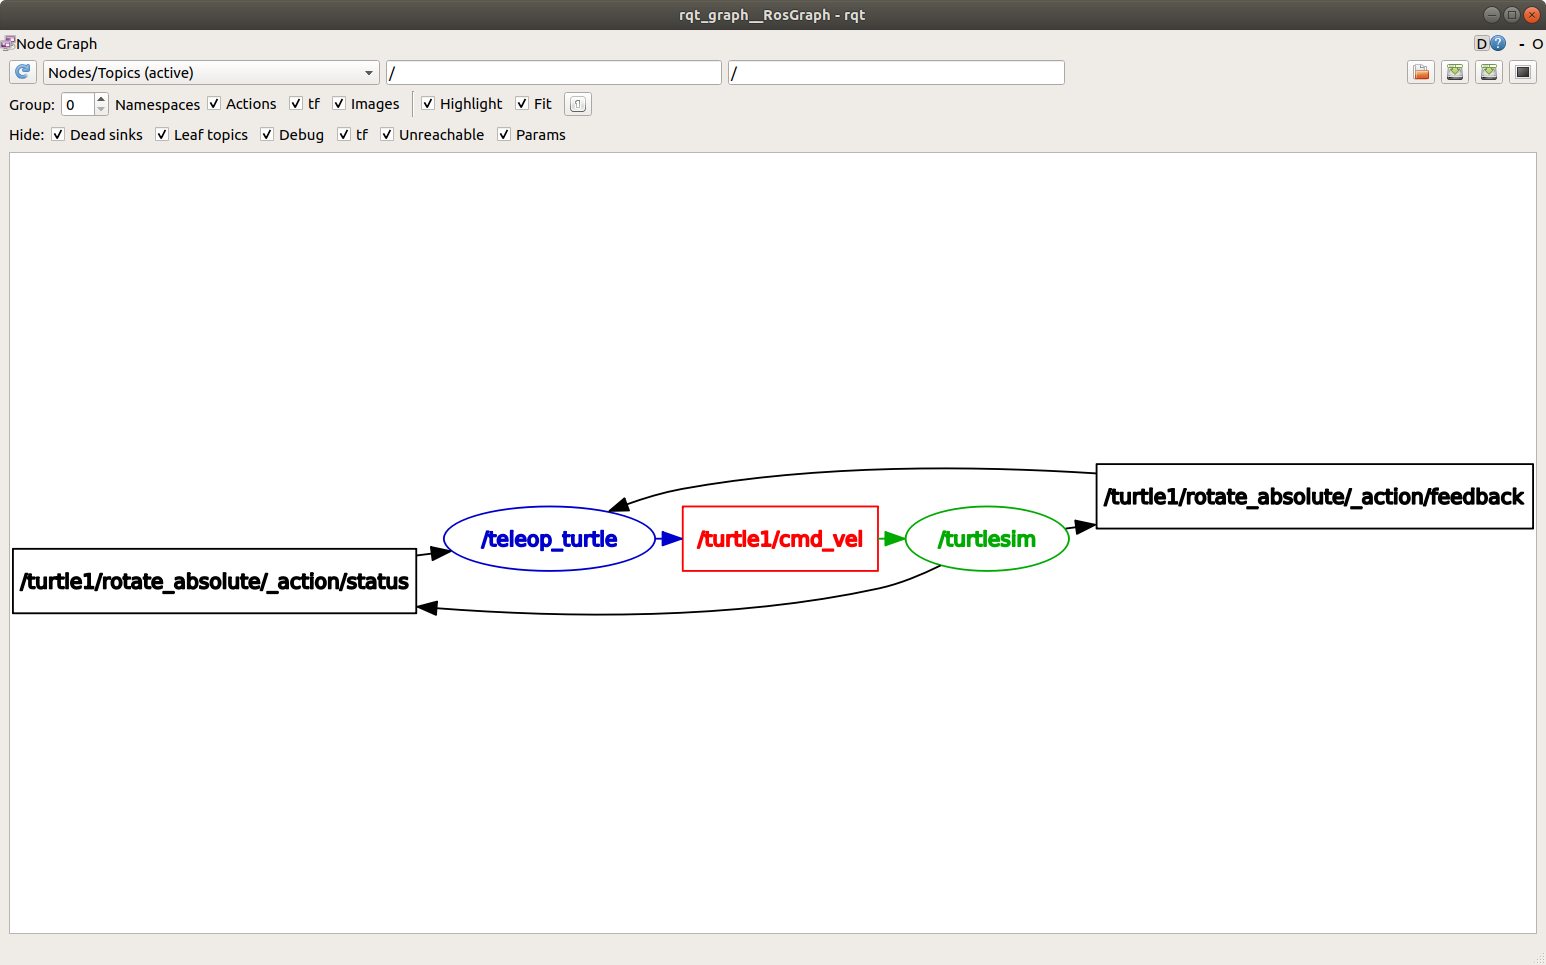
\includegraphics[width=10cm, height=8cm]{rqt-graph.png}
\caption{Esempio concreto di nodi che comunicano attraverso topic grazie allo strumento di ROS 2 rqt_graph}
\label{rqt-g}
\end{figure}

\begin{figure}[!htbp]
\centering
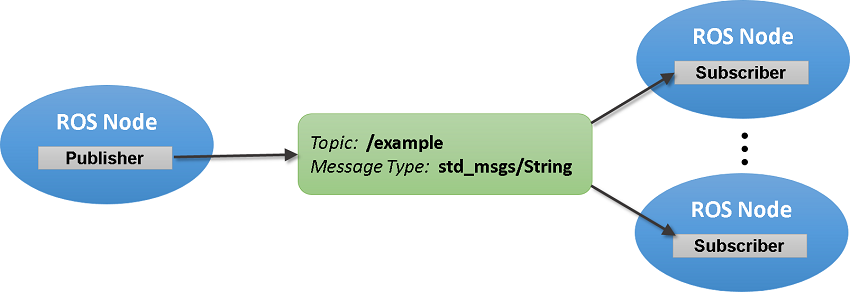
\includegraphics[width=14cm, height=5cm]{pub-sub-topic.png}
\caption{Grafico meccanismo di publish/subscribe}
\label{p/s}
\end{figure}
\vspace{3cm}
\section{Struttura di un ambiente di sviluppo in ROS 2}
L'ambiente di sviluppo per applicazioni di ROS 2 è di fondamentale importanza. Infatti, queste applicazioni devono tenere conto di innumerevoli aspetti e devono poter gestire un'alta quantità di file e risorse.
Per questo hanno una struttura fortemente gerarchica e facilmente intercambiabile.
L'unità base è il workspace, ovvero una directory contenente un insieme di package di ROS 2.
\'E possibile avere più workspaces contenuti fra di loro, denominati meta workspace. Devono avere almeno tutte le dipendenze del workspace che li contiene e  possono sovrascrivere le funzioni del workspace principale.
Ogni workspace invece è composto da molti package. Il package è sostanzialmente il contenitore del codice. \'E fondamentale per organizzare ordinatamente il sistema che si sta sviluppando e per permettere il building separato di parti del progetto. Inoltre a differenza di altri sistemi software in cui ogni sviluppatore lavora ad un package alla volta, sia su ROS che su ROS 2 è normale distribuire il codice in un alto numero di package, secondo il principio di riutilizzo/rilascio.
Tra i linguaggi di programmazione a disposizione per svliuppare un package, i due principali sono C++ e Python. Nel contesto dell'elaborato, uniformenente con la scelta di C++ come linguaggio di programmazione, è stato scelto di utilizzare il sistema di building \emph{ament\_cmake}.
Conseguentemente i due file fondamentali e sempre presenti di un package di ROS 2 sono:
\begin{enumerate}
  \item package.xml: contiene informazioni generali sul progetto e in particolare le dipendenze esterne del tuo package.
  \item CmakeLists.txt: si occupa di trovare le dipendenze richieste dal package e di installare correttamente il package.
\end{enumerate}

Essi sono fondamentali in quanto non solo descrivono il pacchetto e contengono informazioni importanti riguardo a licenza, mantenitori e proprietario ma sono indispensabili per effettuare il building dei package. Infatti dichiarano e definiscono il buildtool utilizzato, dipendenze di package esterni ed informazioni necessarie per poter installare e rendere fruibile il package all'interno di ROS 2.
Oltre ai due file elencati qui sopra ogni package può disporre di una cartella $src$ che contiene i nodi del sistema, una cartella $include$ che contiene i rispettivi file header e altre cartelle contenenti file di lancio, file \emph{.world}, che descrivono il "mondo" della simulazione o file \emph{.urdf}. Nell'ultima sezione del capitolo sarà data una spiegazione più accurata di questi ultimi file.
Come specificato nella sezione precedente è consono decidere di organizzare i progetti di ROS 2 utilizzando molti packages. Questo comporta la necessità di avere un sistema di building efficiente ed elastico che permetta di lavorare con singoli package o molti package contemporaneamente. Su ROS erano disponibili molti sistemi di building che possedevano funzionalità diverse e molto specifiche ma che non garantivano completezza. Da qui è scaturità la necessità di disporre di un unico meccanismo di building completo ed autosufficiente per ridurre i costi di mantenimento dei progetti ed aumentarne la praticità.
In questa direzione è stato sviluppato \emph{colcon}, un sistema di building universale in grado di compilare workspaces di ROS e ROS 2 senza esserne intrinsicamente legato. Esso è infatti adibito all'accensione di Gazebo e alla gestione delle dipendenze dei package necessari per il suo funzionamento.
Per compilare l'intero workspace è necessario lanciare il comando
 \begin{lstlisting}
 colcon build
\end{lstlisting}
 nell'origine del workspace, utilizzando la shell del proprio sistema operativo.
Terminato il building dei package all'interno del workspace saranno state create da \emph{colcon} tre \emph{directory} fondamentali:
\begin{enumerate}
\item la directory \emph{build} contenente i file responsabili del building di ogni package (infatti ci sarà una sottocartella per ogni package all'interno del workspace)
\item la directory \emph{install}, dove saranno effettivamente installati i package
\item la directory  \emph{log} responsabile di diversi file di log riguardanti la fase di building svolta da \emph{colcon}.
\end{enumerate}

\'E possibile eseguire singolarmente ogni nodo del sistema, ma l'aumento dei nodi creerebbe una situazione particolarmente difficile
da gestire se affidata unicamente al lancio di ogni nodo singolarmente. È quindi stato sviluppato un sistema di file di lancio con il quale diversi nodi possono essere lanciati su ROS 2 con specifici parametri di inizializzazione e con la possibilità di richiamare altri file di lancio. Il launch file di ROS 2 è anche responsabile del monitoraggio dello stato dei processi lanciati, riportando o reagendo a cambienti nello stato del processi. Inoltre è utilizzabile per lanciare Gazebo e caricare il modello \emph{URDF} del robot all'interno della simulazione. Su ROS 2 è realizzato tramite \emph{Python} e il package che si occupa della fase di lancio è \emph{launch_ros}.
Dopo il building del progetto con \emph{concon build}, è possibile lanciare l'intero progetto composto da diversi nodi con un semplice comando di cui ne viene riportato un semplice esempio:
\begin{lstlisting}
ros2 launch myPackage script.launch.py
\end{lstlisting}

La comunicazione all'interno di ROS 2 si basa su un \emph{DDS} (Data Distributed Service)\footnote{\url{https://design.ros2.org/articles/ros_on_dds.html}}. Il DDS è un middleware, che gestisce un complesso sistema
di scambio messaggi basato sul paradigma publish/subscribe . Erede del server "Master" di ROS 1, sulla scia di un server RPC, il DDS permette la definizione di messaggi, la loro serializzazione e deserializzazione garantendo
il corretto funzionamento del meccanismo di publish/subscribe. 
Per massimizzare l'esperienza degli utenti e per facilitare l'ingresso nella comunità, ROS 2 provvede a fornire delle interfacce simili a ROS che nasconderanno la maggior parte della complessità, ma che contemporaneamente metteranno a disposizione API per l'accesso al DDS per utenti con necessità molto stringenti o per integrazioni con altri sistemi DDS, come è visionabile dalla figura\ref{DDS}.
Il DDS si occupa anche di mantenere il formato \emph{.msg} nella comunicazione tra nodi. Per poter essere utilizzato però deve essere convertito nel formato \emph{.idl}, un formato a campi utilizzato dal DDS per trasportare più valori in un singolo messaggio. E' stato verificato tramite esperimenti empirici che la conversione e riconversione attuata dal DDS per trasportare i messaggi è più efficace della serializzazione e invio di ciascun campo.

\begin{figure}[htbp]
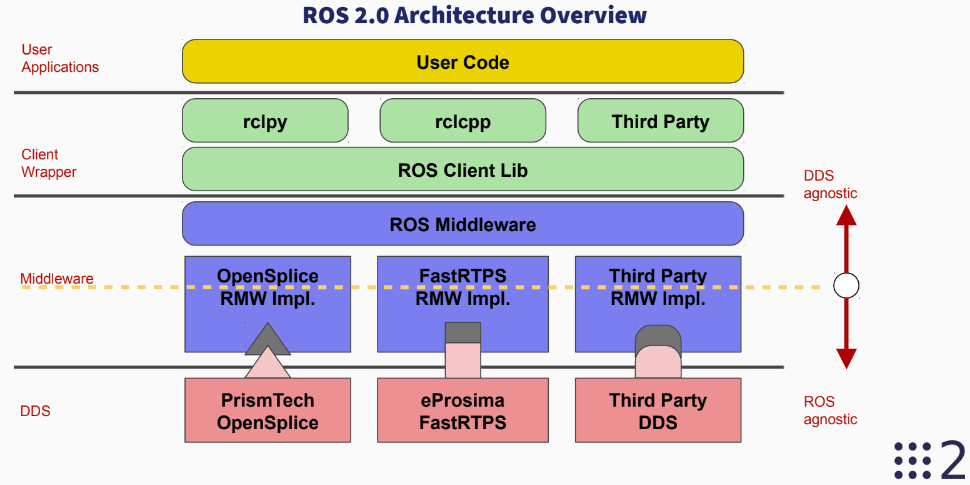
\includegraphics[width=12cm, height=8cm]{DDS2.png}
\caption{Relazione tra stack di ROS 2 e il DDS sottostante}
\label{DDS}
\end{figure}

Strettamente legata al DDS e ai servizi offerti la QualityofService (QoS) è un parametro fondamentale per gestire il
livello di qualità di trasmissione dati dei nodi e quindi del sistema generale. Calibrando il livelo del QoS
possibile diverse tipologie di connesione che possono passare da un TPC a diverse
gradazioni di un UDP best effort. Diversamente da ROS, permette di scegliere il livello di affidabilità della comunicazione in base alla tipologia di situazione che si sta affrontando: da comunicazioni UDP con un minor grado di responsabilità ad ambienti real-time con tempistiche più stringenti. I parametri fondamentali che caratterizzano la QoS sono:
\begin{enumerate}
\item history: rappresenta la tipologia di salvataggio dei dati che può comprendere tutti i samples scambiati o solamente di un numero N
\item depth: Se i campioni vengono salvati in un numero finito allora il parametro rappresenta l'effettivo numero.(Nel caso il salvataggio sia totale allora è un parametro superfluo).
\item affidabilità: può essere "best effort" o "Reliable" e indica se verrà applicato un protocollo basato su UDP o su TCP
\item durabilità: indica la possibilità da parte del publisher di salvare i dati per eventuali "late-joining" iscrizioni.
\item deadline: il limite massimo di ogni dato per essere pubblicato.
\item livilness: la durata per cui un nodo è considerato ancora "vivo", cioè che può pubblicare dati in un topic.
\end{enumerate}

\vspace{20mm}
\vspace{20mm}
\vspace{20mm}
\vspace{20mm}
\vspace{20mm}
\vspace{10mm}
\vspace{10mm}
\vspace{10mm}
\vspace{10mm}
\vspace{10mm}
\vspace{10mm}
\vspace{10mm}


\section{GAZEBO E URDF}
Gazebo\footnote{\url{http://gazebosim.org/tutorials}} è un simulatore dinamico 3D con la capacità di simulare efficientemente robot in complessi ambienti indoor o outdoor. E' solitamente usato per testare algoritmi su robot, per progettare il design e testarne l'affidabilità in ambienti realistici.
Ciò è reso possibile da un ampio set di librerie di modelli e ambienti, un'importante disponibilità di sensori e soprattutto interfacce grafiche molto convenienti gestite da Gazebo Server, il processo che si occupa di utilizzare i file di configurazione di Gazebo per produrre la simulazione.
Il primo componente fondamentale è il file \emph{world}, che contiene la descrizione del mondo e degli oggetti presenti in una simulazione. Incorpora la descrizione dei robot, degli scenari, eventuali luci e un'ampia gamma di sensori concreti di ampia diffusione nel mercato.
Successivamente è importante definire il robot che viene utilizzato nella simulazione ed è necessario comporlo in maniera realistica, per garantire una simulazione concreta ed efficiente. Da questa necessità è nato URDF\footnote{\url{http://wiki.ros.org/urdf/}}(Universal Robotic Description Format), un formato XML usato su ROS 2 e ROS per descrivere gli elementi costituivi di un robot, come essi sono collegati tra di loro e le loro proprietà fisiche.
Per esempio, un corpo è definito dal tag $link$ e al suo interno può definire molte proprietà geometriche, sul materiale o che permettono di definire una gerarchia tra i componenti seguendo una struttura ad albero. Ma il parser che analizza il file URDF non sa la precisazione ubicazione del componente. Per definire il collegamento con altri link è necessario inserire il tag $<joint>$, il quale permette di definire l'unione concreta tra due componenti. Utilizzando questi tag principali è facile costruire le basi di qualsiasi robot come è visibile in figura \ref{urdf}.
All'aumentare del numero di link e di joint del sistema, la complessità del file aumenta considerevolmente e per alleggerire il codice e per evitarne la ripetizione è stato ideato un sistema di scripting per file URDF denominato XACRO\footnote{\url{http://wiki.ros.org/xacro}}. Esso permette la definizione di costanti, ovvero di definire un componente noto del robot sotto uno specifico nome, in modo da non doverlo definire più volte. Ma può anche intervenire a livello matematico, permettendo il calcolo di espressioni che rendono più elastico il design del robot. Infine è molto pratico in quanto permette la definizione di macro, che definiscono componenti attraverso parametri. Se per esempio dovessero servire due gambe speculari, sarebbe possibile crearne due tramite una semplice dichiarazione, riempendo un campo con \emph{left} o \emph{right}.
Per poter integrare le descrizioni dei robot del linguaggio URDF è fondamentale l'elemento $gazebo$ che permette di aggiungere specifiche proprietà al robot, necessarie per il corretto funzionamento all'interno della simulazione .
Infatti è possibile integrare al file URDF, di descrizione fisica del robot, una serie di plugin base di Gazebo o una loro estensione creata dall'utente.
Un plugin è un pezzo di codice che è compilato ed inserito all'interno della simulazione che ha accesso a tutte le funzioni di Gazebo.
I plugins sono particolarmente utili per:
\begin{itemize}
  \item lasciare ad ogni sviluppatore pieno controllo della simulazione
  \item perchè sono inseribili o disinseribili dal sistema in stato di running
  \item estremamente flessibili
  \item rappresentano una comoda interfaccia per Gazebo che non produce un eccessivo overhead per la serializzazione e deserializzazione dei messaggi
\end{itemize}
Ci sono 6 tipologie di plugins disponibili:
\begin{itemize}
  \item World
  \item Model
  \item Sensor
  \item System
  \item Visual
  \item GUI
\end{itemize}
Ogni plugin è gestito da un differente componente di Gazebo. Un WorldPlugin sarà legato ad un world di Gazebo, mentre un ModelPlugin sarà coinvolto da un file che descrive un modello di robot.
Gli esempi fondamentali utilizzati nel nostro caso di interesse sono \emph{differential_drive_controller} che fornisce un controllo basico di un robot a ruote differenziali da parte di Gazebo.
Garantisce alcune funzionalità fondamentali:
\begin{enumerate}
\item può definire il topic da cui leggere la velocità da riprodurre nella simulazione.
\item  scegliere il riferimento in base al quale pubblicare odom(ovvero la posizione nel sistema di riferimento assoluto della simulazione).
\end{enumerate}
In conclusione è citato il Gazebo Master, parte fondamentale su cui si basa Gazebo.
Provvede a gestire i topic, garantire la corretta traduzione dalla tabella di lookup e si occupa delle librerie per la comunicazione tra nodi.
Provvede anche a definire i comportamenti fisici che garantiscono realisticità e concretezza degli oggetti e dei loro comportamenti durante l'interazione con altri elementi della simulazione. Inoltre dispone di librerie per il renderning 3D delle scene nella GUI e della loro riproduzione nel simulatore.
\\
\\
Gazebo risulta un'applicazione stand-alone ma con una forte dipendenza con ROS e ROS 2 grazie ad un set di packages chiamati \emph{gazebo_ros_pkgs} nei quali si crea un ponte tra le API di Gazebo e il meccanismo dei messaggi di ROS 2.
I packages più importanti da citare e maggiormente fondamentali per lo sviluppo di un'applicazione robotica sono:
\begin{enumerate}
\item gazebo_ros_pkgs: un metapackage contenente diversi package di utilità.
Si rivelano molto importanti gazebo_dev che fornisce una configurazione di default di Gazebo per le distribuzioni di ROS.
\item gazebo_msgs: predispone strutture dati utili alla comunicazione tra Gazebo e ROS 2.
\item gazebo_ros:  convenienti funzioni utilizzabili da plugin.
\item gazebo_plugins: ovvero una serie di plugings di Gazebo che emulano sensori per ROS 2.
\end{enumerate}

Le differenze fondamentali nell'utilizzo di Gazebo tra ROS a ROS 2 sono:
\begin{enumerate}
\item lo sfruttamento pieno delle nuove ricche specifiche di ROS 2, come l'assenza del server master.
\item la standardizzazione di funzionalità comuni, come il namespace di ROS, parametri e rimappatura di topic
\item la modernizzazione del codice, grazie alla possibilità di riscrivere il codice URDF esisten con l'ultimo formato \emph{SDF}
\end{enumerate}

\begin{figure}[!ht]
\centering
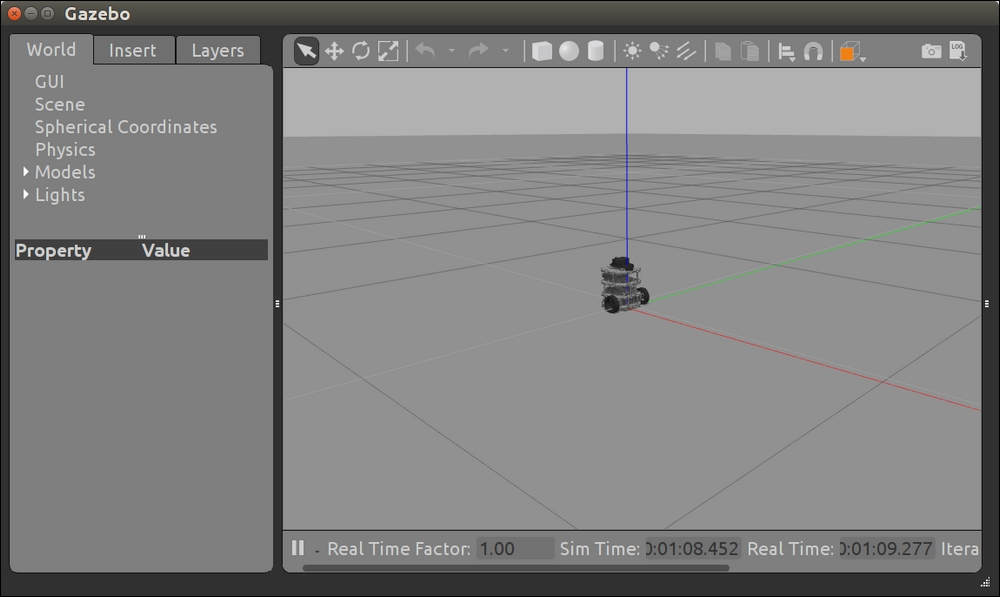
\includegraphics[width=14cm, height=8.5cm]{gazebo1.jpg}
\caption{Esempio simulazione robot in un mondo vuoto con Gazebo}
\label{fig}
\end{figure}

\begin{figure}[!ht]
\centering
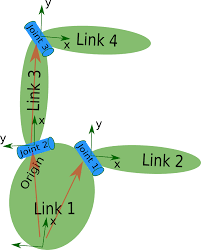
\includegraphics[width=5cm, height=8cm]{urdf1.png}
\caption{Esempio concreto della composizione di un robot tramite link e joint}
\label{urdf}
\end{figure}

\chapter{Modellazione e controllo di un uniciclo}

Un uniciclo è un veicolo avente una sola ruota orientabile, che generalmente si muove in solo due dimensioni dello spazio con una velocità di spostamento laterale nulla.
Nonostante il nome "uniciclo" nella realtà i sistemi con una sola ruota sono particolarmente instabili, di conseguenza in molte situazioni, questo modello può descrivere, seppur in maniera approssimata, modelli di robot a due ruote o modelli semplici di automobili.

\section{Modello matematico}
In questa sezione, considereremo il modello matematico di un robot che si muove nel piano $\{x,y\}$. Nel seguente scenario, è possibile descrivere il suo orientamento utilizzando un solo angolo denominato $\delta$. Il modello matematico risulta dunque:
%
\begin{equation*}
\begin{bmatrix}
\dot{x}\\
\dot{y}\\
\dot{\delta}
\end{bmatrix}=\begin{bmatrix}
v\cos(\theta)\\
v\sin(\theta)\\
\omega
\end{bmatrix},
\label{modello}
\end{equation*}
%
dove $v$ è la velocità lineare del robot mentre $\omega$ è la velocità angolare del robot lungo l'asse uscente dal piano $\{x,y\}$.
Si rimanda il lettore a \ref{uniciclo} per una rappresentazione grafica.
Nel seguito, si rappresenta come $\delta\in(-\pi,\pi]$ l'orientamento che ha il
robot rispetto alla linea di congiunzione tra il robot stesso e il punto di arrivo desiderato. Inoltre, si definisce $\theta\in(-\pi,\pi]$ l'orientamento desiderato del robot quando si trova nella posizione $T$. Infine, si definisce $r\in\mathbb{R}_{\geq 0}$ la distanza tra il robot e il target nel piano $\{x,y\}$. Si rimanda il lettore alla \ref{uniciclo} per una rappresentazione grafica.
\\
\begin{figure}[!htbp]
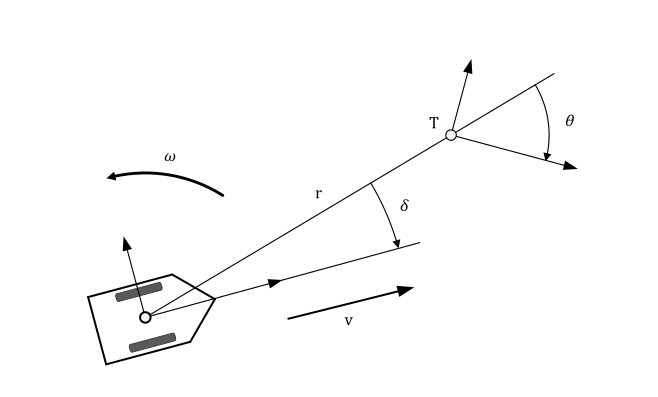
\includegraphics[width=12cm, height=8cm]{coordinate-sistema.png}
\caption{Modello dell'uniciclo}
\label{uniciclo}
\end{figure}

Si può quindi scrivere la legge cinematica del veicolo rispetto al robot come:
\begin{align}\
\begin{bmatrix}
  \dot r\\ 
  \dot{\theta}\\
  \dot{\delta}
\end{bmatrix} =
\begin{bmatrix}
  -v \cos\delta\\ 
  \frac{v}{r}\cdot\sin(\delta)\\
  \frac{v}{r}\cdot\sin(\delta) + \omega\\
\end{bmatrix}
\end{align}


\section{Controllore}
Lo scopo di questa sezione è descrivere la legge di controllo per l'uniciclo che sarà poi implementata in un'architettura tramite ROS 2. Nel seguente elaborato, l'obiettivo è far raggiungere al robot un punto $T$. La legge di controllo è basata su una rappresentazione in coordinate polari della posizione del punto target rispetto al veicolo. Per questo motivo, la legge di controllo è anche detta \emph{egocentrica}. Questo cambio di coordinate, come motivato anche in \cite{CONTROLLO:1}, permette di implementare una legge di controllo senza discontinuità e che si avvicina all'esperienza di guida di un pilota umano.
L'obiettivo della legge di controllo è ridurre la distanza $r$ tra il robot e il punto di arrivo $T$ e portare il robot a orientarsi ad un angolo $\theta$.
Partendo dall'osservare l'equazione \eqref{modello} si può notare che, considerando $v$ strettamente maggiore di zero e $\omega$ l'unica variabile di controllo, allora $\omega$ controlla unicamente lo stato $\delta$, mentre $(r,\theta)^{T}$ sono determinate da $\delta$. Inoltre la sola coppia  $(r, \theta)^{T}$ descrive la posizione del veicolo, mentre $\delta$ corrisponde al suo sterzo. Per cui è sensato  dividere in due il sistema ottenendo:

\begin{align}
\begin{bmatrix}
  \dot r\\ 
  \dot{\theta}
\end{bmatrix}
 =
\begin{bmatrix}
  -v \cos\delta\\ 
  \frac{v}{r}\cdot\sin\delta\\
\end{bmatrix}
\end{align}
\begin{align}
\dot{\delta} = \frac{v}{r}\cdot\sin(\delta) + \omega
\end{align}
\vspace{1mm}

Si può quindi notare che ci sono due variabili di controllo, la prima corrisponde a $\delta$, che guida il sotto sistema dell'equazione (2.2) verso l'origine e un controllore effettivo $\omega$ che rende la dinamica del sottosistema (2.3) più veloce rispetto al sistema (2.2) e stabilizza $\delta$ come un controllo virtuale. Per cui (2.2) diviene un sostto sistema lento e (2.3) diventa un sottosistema veloce a singola perturbazione. La divisione di questi due sistemi rende facile lo spostamento del robot nella posizione-target predefinita con il giusto assetto.
\\
Per quanto riguarda il sottosistema lento, come dimostrato in \cite{CONTROLLO:1}, prendendo una semplice funzione Lyapunov:
\begin{align}
 V = 1/2\cdot(r^2 + \theta^2)
\end{align}

e considerando il controllo virtuale con $k_1 > 0$ e costante
\begin{align}
 \delta = \arctan(-k_1\cdot\theta)
\end{align}

derivando la funzione di Lyupanov si ottiene che il controllo virtuale $\delta$ sterza il sistema dalla posizione iniziale verso l'origine e che è negativa in tutti punti tranne l'origine, quindi è considerabile stabile.
Considerando che l'arcotangente è una funzione liscia e che  $\texttt{arctan}(0)=0$ allora avremo che se $\theta\to 0$ allora $\delta \to 0$ e che conseguentemente $(r,\theta,\delta)^{T}$ si dirige verso l'origine. Inoltre scegliendo $v$ in modo tale da eliminare il punto di singolarità in $r$ si ottiene che l'origine è globalmente stabile.
In seguito è da sviluppare una legge di controllo per lo sterzo del veicolo.
Supponiamo $z$ la differenza tra lo stato attuale $\delta$ e la proprietà desiderata $\arctan(-k_1\theta)$, tale che:
\begin{align}
z\equiv\delta - \arctan(-k_1\theta)
\end{align}

Derivando rispetto al tempo, è possibile dimostrare che la seguente scelta di $\omega$ stabilizza l'errore $z$ a $0$.
\begin{align}
\omega = \frac{-v}{r} \left[ k_2\cdot + (1 + \frac{k_1}{1+ (k_1\theta)^2}k_1+(k_1\theta)^2)\cdot\sin(z + \arctan(-k_1\theta)) \right] 
\end{align}
che nelle coordinate originali, esplicitando l'input ovvero $\omega$ risulta la legge di controllo per $\omega$:
\begin{align}
\label{cont-law}
\omega = \frac{-v}{r} \left[ k_2(\delta - \arctan(-k_1\omega)) + (1 + \frac{k_1}{1 + (k_1\omega)^{2}})\sin\delta) \right]
\end{align}

Si evince che abbiamo $v$ come variabile libera e che la forma della traiettoria non dipende da essa.
Ma come è stato precedentemente la convergenza asintotica del robot al punto previsto dipende dalla scelta della velocità intorno all'origine. È globalmente asintotica solo se $v\to 0$ per $r \to 0$.  
Questa scelta di $\omega $ e $v$ rende quindi possibile controllare un uniciclo verso un punto $T$ desiderato e con un certo assetto. 


\chapter{Implementazione e risultati}
In questo capitolo, verrà descritta in maniera dettagliata l'implementazione del controllore definito nel capitolo precedente, attraverso ROS 2 e i relativi strumenti spiegati nel primo capitolo. Vengono inoltre descritti e commentati i risultati ottenuti dall'implementazione attraverso un insieme di plot e immagini dimostrative. Per l'implementazione è stato utilizzato \emph{ROS 2 Eloquent} per \emph{Ubuntu Bionic}. Come meglio approfondito nel capitolo il robot utilizzato per effettuare gli esperimenti è il \emph{TurtleBot3Burger}.


\section{Implementazione}
Per l'implementazione del controllore è stato deciso di seguire la struttura classica delle applicazioni robotiche. Generalmente, è una struttura formata da due unità fondamentali, la cui cooperazione risulta necessaria per una guida efficente.
Le due entità sono \emph{pianificatore} e \emph{controllore}. Il controllore è l'unità che implementa la legge di controllo e che quindi gestisce la correttezza della traiettoria tra il punto iniziale fino alla destinazione $T$ e il giusto assetto finale. Invece il pianificatore sceglie il suddetto punto $T$ e l'orientamento per una navigazione ottimizzata. Esso comunica le coordinate al controllore e riceve feedback riguardo il successo dell'operazione, e molto spesso anche informazioni durante il tragitto stesso. Questa struttura a moduli distinti è estremamente efficace, in quanto una modifica del controllore o la sua sosituzione con una legge di controllo differente non comprometterebbe la riscrittura del pianificatore. Intuivamente anche se il pianificatore fosse scambiato o modificato, il controllore rimarrebbe immutato.
Come prima operazione è stato dunque creato un ROS 2 package chiamato \emph{position_controller} nel quale inserire controllore e pianificatore.
Il paradigma \emph{pianificatore-controllore} è stato implementato utilizzando due distinti nodi di ROS 2 ed è stato utilizzato C++ per ottenere la massima efficienza.
Sono stati dunque creati due file per controllore e pianificatore chiamati rispettivamente:
\begin{lstlisting}
controllore.cpp 
pianificatore.cpp
\end{lstlisting} 
inseriti nella cartella $src$ del package.
Inoltre, come usuale in applicazioni create con C++, è stato diviso il funzionamento dalla parte di richiamo delle librerie, per questo sono stati creati altri due file denominati
\begin{lstlisting}
controllore.hpp 
pianificatore.hpp
\end{lstlisting}
dove sono state inserite le dichiarazioni di tutte le variabili e dei metodi utilizzati nel corrispettivo file \emph{.cpp}.

Sono stati creati due topic per garantire la comunicazione della posizione e la conferma del suo raggiungimento. Il primo  è stato chiamato $position$ ed è dove è stata pubblicata la terna di valori che specifica la posizione e l'assetto finale target. Il messaggio $position$ viene letto rapidamente dal controllore che successivamente elabora la strategia più adatta tramite la legge di controllo. Quando il controllore rivela che il robot ha raggiunto il punto desiderato pubblica l'esito del tragitto  sul topic $response$, da lui creato, che corrisponderà a fallimento o successo.
I messaggi $position$ e $response$ sono stati definiti in un package a parte specifico per la definzione di messaggi denominato come $position\_controller\_msgs$.
Il messaggio $response$ è stato definito:
\begin{lstlisting}
float64 posx 
float64 posy
float64 postheta
\end{lstlisting}
utilizzando dei \emph{float64} per garantire un'accuratezza massima, mentre $position$ è stato semplicemente definito come:
\begin{lstlisting}
bool resp
\end{lstlisting}
dove il valore \emph{true} corrisponderebbe al successo dell'operazione mentre \emph{false} all'insuccesso.

La QoS di ROS 2 utilizzata per la creazione di questi due topic è stata pensata per ottenere una comunicazione estremamente sicura in quanto la perdita della posizione successiva o il mancato arrivo della conferma della posizione da parte del controllore metterebbe in stallo l'applicazione.
È stata data una particolare attenzione all'integrità dei messaggi trasmessi sul DDS. Per questo il protocollo di comunicazione usato è \emph{TCP/IP}, il quale garantisce l'arrivo completo dei messaggi inviati. Inoltre è stato deciso di mantenere una storia di dieci messaggi per ottenere un grado di sicurezza ancora più elevato. Naturalmente, se l'architettura venisse riutilizzata in una diversa applicazione, in cui fosse necessario un livello di sicurezza di scambio di messaggi maggiore, allora entrerebbero in gioco altri parametri descritti nel capitolo precedente. Viceversa se l'architettura venisse utilizzata in un contesto più dinamico, con una maggiore predilizione all'arrivo del messaggio nel minor tempo e con costi minimi rispetto alla sua integrità verrebbe utilizzata una comunicazione UDP best effort o probabilmente sarebbero considerati parametri come \emph{deadline} o \emph{livilness}.


\subsection{Pianificatore}
Come accennato precedentemente il pianificatore è composto da un file \emph{.cpp} e da un file \emph{.hpp}. Nel file header sono stati incluse le principali librerie per il funzionamento del pianificatore.
Oltre alle consuete librerie di I/O, ed espressioni matematiche le fondamentali sono le librerie per i messaggi della posizione target, il messaggio di conferma per il pianificatore, l'header del messaggio odom ed in particolare rclcpp, necessaria per la creazione di nodi e iscrizione o creazione di topic.
Infine è stata dichiarata la classe \emph{Pianificatore} derivata da \emph{rclcpp::Node}, la quale ottiene tutte le peculiarità di un nodo di ROS 2.
\\
Il file $pianificatore.cpp$ invece è composto da un breve $main$ che si occupa di inizializzare gli argomenti passati come parametri, di lanciare la classe rappresentatante il nodo e di eliminare il nodo stesso al termine della sua esecuzione liberando la memoria e le restanti risorse utilizzate.
Il pianificatore, nella sua fase di inizializzazione crea un oggetto publisher che può pubblicare sul topic $position$, mentre si iscrive al topic \emph{Response} che invece indica l'esito del controllore. Il subscriber ha un comportamento asincrono, in quanto un messaggio su un topic può essere pubblicato in qualsiasi momento senza una logica stringente, per questo ad esso viene associato una funzione di callback eseguita ogni volta che il subscriber legge un messaggio sul topic di interesse. Nel caso del pianificatore la funzione di callback riceve l'esito dell'obiettivo imposto ed analizza la risposta. Se il responso è positivo inizializza un messaggio \emph{Position} e inserisce la terna $(x,t, \theta)$, ovvero le coordinate del piano \emph{(x,y)} con l'assetto desiderato.
Infine con l'oggetto publisher precedentemente creato pubblica sul topic il messaggio, il quale è letto dal nodo rappresentante il  controllore. Successivamente il controllore pubblica sul topic \emph{response} il valore che può essere \emph{true}, se è stato raggiunto l'obiettivo o \emph{false} se l'obiettivo è fallito.
\subsection{Controllore}
Come per il pianificatore anche il controllore richiama nel file header tutte le comune librerie fondamentali di I/O, su funzioni matematiche e riguardanti sistema operativo. Le più rilevanti per la struttura del progetto con ROS 2 sono \emph{odometry}, contenente il messaggio sulle coordinate assolute del robot, \emph{tf2} , per effettuare trasformazioni dal sistema di riferimento assoluto al sistema di riferimento del robot, e \emph{twist} un messaggio che definisce le componenti della velocità nello spazio.
Il controllore crea un subscriber sul topic \emph{Position}, per leggere dal pianificatore la terna $(x,t, \theta)$, mentre viceversa rispetto al pianificatore pubblica sul topic \emph{Response} per confermare l'avvenuta ricezione del punto o un eventuale errore se il procedimento non avvenisse correttamente, come se per esempio il messaggio pubblicato sul topic \emph{Position} non fosse composto da tre valori, o se il robot non fosse riuscito ad arrivare a destinazione.
Come seconda operazione il controllore crea un subscriber per il topic \emph{odom}. Il topic odom è fondamentale, in quanto rappresenta la posizione in coordinate assolute di un punto all'interno alla simulazione.
Seppure l'aggiornamento di odom molto frequente, la pubblicazione è asincrona ed è quindi necessario associargli una funzione di callback denominata $odom\_callback$.
La funzione di callback riceve il messaggio da odom il quale è composto da una quaterna di valori $(x,y,z,\omega)$. In seguito viene utilizzata la libreria \emph{tf2} che prende in ingresso i valori del messaggio \emph{odom}, produce un quaternione, crea la rispettiva matrice di rotazione e da essa ottiene il valore in radianti della rotazione del robot rispetto ai tre assi cartesiani utilizzando il metodo $getRPY(roll, pitch, yaw)$. I valori roll e pitch in condizioni normali sono trascurabili in quanto non è prevista nessuna rotazione rispetto all'asse x e y. Viene solamente effettuato un breve controllo, intuitivo ed immediato per verificare che il robot non sia ribaltato, mentre come visibile in figura \ref{quaternione}, \emph{yaw} corrisponde al valore della rotazione intorno all'asse z del robot con odom come riferimento.
\\
La legge di controllo è implementata nel metodo \emph{update_callback}, sul quale è impostato un timer di \emph{100 ms}, ovvero il periodo ogni quanto il nodo esegue esegue periodicamente la funzione. All'interno di \emph{update_callback}, dopo aver ottenuto almeno una volta il valore di odom e la posizione target attravero il topic \emph{request}, vengono calcolati le variabili necessarie per applicare la legge di controllo (2.5) sulla velocità angolare $\omega$.
Considerando \emph{goal_pose_x} e \emph{goal_pose_y} la posizione target sul piano $\{x,y\}$ e $last\_pose\_y$ , l'ultima posizione ricevuta dal topic \emph{odom}, allora definiamo $path_theta$ come:
\begin{lstlisting}
 path_theta = atan2(goal_pose_y-last_pose_y, goal_pose_x -last_pose_x);
\end{lstlisting}
ovvero l'angolo compreso tra la congiungente tra il robot e la posizione target e il sistema di riferimento.
Successivamente definendo $last\_pose\_theta$ come l'orientamento del robot più recente ricevuto da odom, calcoliamo $\delta$ ovvero l'orientamento che ha il robot rispetto alla linea di congiunzione tra il robot stesso e il punto desiderato:
 \begin{lstlisting}
 delta = last_pose_theta - path_theta
  \end{lstlisting} 
In seguito viene calcolata la distanza tra la posizione attuale e il punto $(x, y)$ desiderato: 
 \begin{lstlisting}
 distance = sqrt(pow((goal_pose_x-last_pose_x),2)+ (pow(goal_pose_y-last_pose_y,2))); 
\end{lstlisting} 
ed in conclusione viene calcolata la legge di controllo come in \eqref{cont-law}
\begin{lstlisting}
twist.angular.z= -((vel/distance)*((k2*(delta-(atan(den))))+(sin(delta)*(1+(k1/den2)))));
\end{lstlisting}

Come spiegato nel precedente capitolo la legge di controllo è applicata alla velocità angolare $\omega$. Nell'implementazione essa corrisponde al messaggio \emph{geometry_msg::msg::Twist} ed in particolare alla velocità angolare rispetto all'asse z.
La velocità lineare del robot $v$, rappresentata da \emph{twist.angular.x} è stata mantenuta costante a $0.2\frac{m}{s}$, ovvero la velocità limite del robot, fino a quando non è stata raggiunta la distanza margine di $1$ m, dalla quale è stata settato lo stesso valore della distanza dalla posizione target, per ottenere un rallentamento uniforme e controllato. Da notare che in questo caso, come si può intuitivamente notare da \eqref{cont-law}, il numeratore annulla il denominatore evitando sbalzi di velocità angolare improvvisi per valori di \emph{distance} molto piccoli. 
Infine il messaggio twist è stato pubblicato sul topic \emph{cmd_vel} letto dal plugin, che si occupa di attuare il movimento.
In definitiva il robot inizia il tragitto e una volta raggiunta la distanza margine incomincia a deccelerare arrivando nella posizione $T$ con l'assetto richiesto.
\\
Per quanto riguarda l'avvio dell'applicazione è stato definito un sistema di lancio all'interno del package $position\_controller$ formato da due file. Il primo è stato denominato  \emph{empty_world.launch.py} e si occupa dell'avvio di Gazebo, caricando il file \emph{world} rappresentante il mondo vuoto e il modello URDF del robot interessato. Infine lancia il secondo file di lancio denominato\emph{robot_state-publisher.launch.py} che invece attiva \emph{robot_state_ publisher} e i due nodi protagonisti dell'architettura ovvero \emph{controllore} e \emph{pianificatore}.
Per lanciare dalla shell si utilizza il comando:
\begin{lstlisting}
ros2 launch position_controller empty_wolrd.launch.py
\end{lstlisting}
Naturalmente nel caso si volesse testare l'architettura con un diverso ambiente dela simulazione o un robot differente, basterebbe cambiare rispettivamente il file \emph{world} e il modello \emph{URDF}.
Infine con il comando \emph{rqt_graph}, messo a disposizione da ROS 2, otteniamo una panoramica generale di nodi e topic attivi durante l'esecuzione nella architettura studiata nell'elaborato come visionabile nella figura \ref{rqt-graph}.

\begin{figure}[htbp]
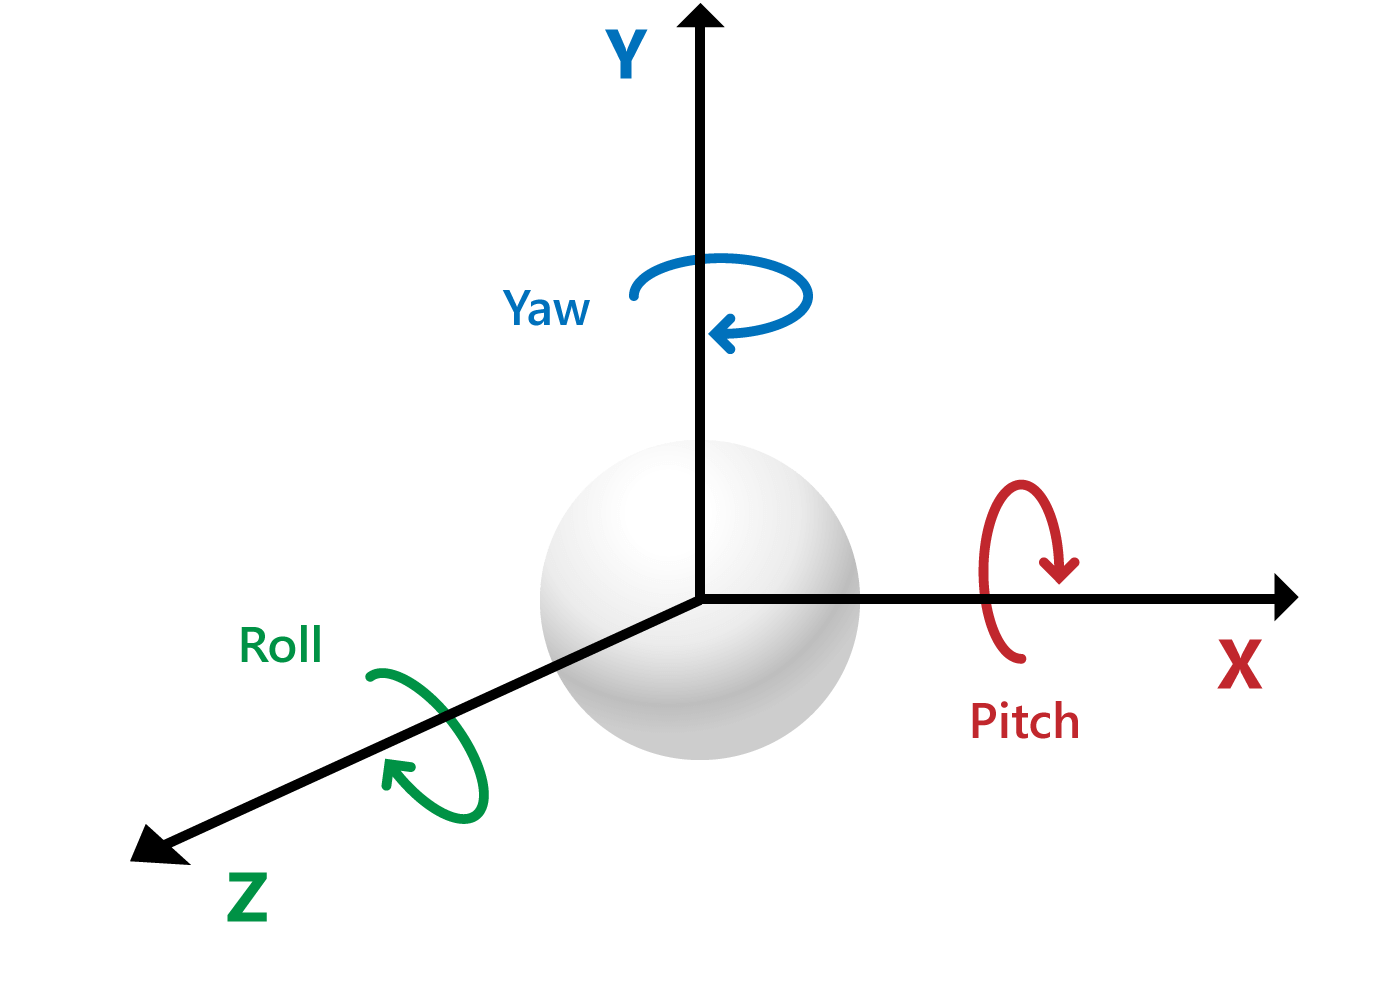
\includegraphics[width=10cm, height=7.5cm]{quaternione.png}
\centering
\caption{Definizione degli angoli di roll, pitch e yaw}
\label{quaternione}
\end{figure}
\begin{figure}[htbp]
\centering
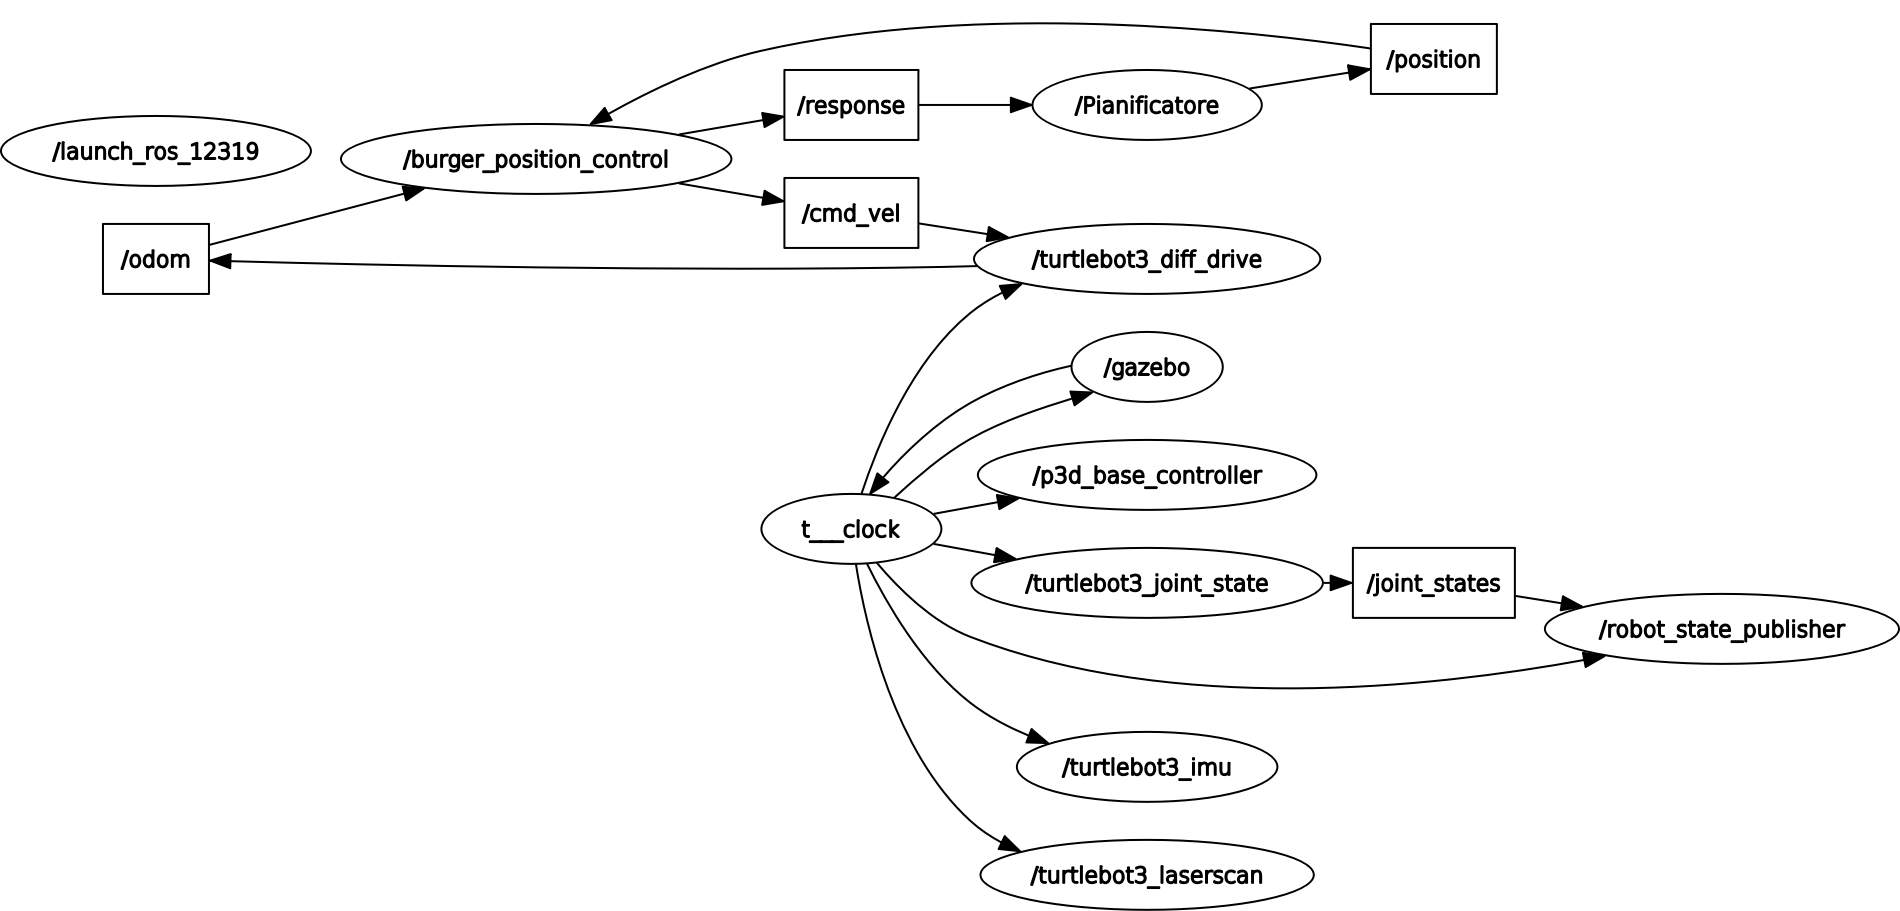
\includegraphics[width=13cm, height=8.5cm]{rosgraph.png}
\caption{Insieme di nodi e topic attivi durante l'esecuzione dell'architettura}
\label{rqt-graph}
\end{figure}
\vspace{5cm}


\subsection{TurtleBot 3}

Il robot terrestre utilizzato per eseguire l'esperimento è il TurtleBot 3 \footnote{\url{https://emanual.robotis.com/docs/en/platform/turtlebot3}} modello Burger, uno dei tre modelli appartenenti alla terza serie dei TurtleBot prodotti da Robotis.
È una piattaforma completamente basata su ROS e su ROS 2 e viene utilizzata per scopi educativi, ma anche commerciali e di ricerca. È un robot mobile semplice, facilmente estendibile, il cui obiettivo pricipale è di compattare le risorse e di ridurre i costi all'essenziale senza perdere di efficienza e produttività. Come è visibile nell'immagine sottostante, dispone di una telecamera LiDAR per la navigazione SLAM e come computer di bordo dispone di un Rasberry Pi 3 affiancato dal modulo di controllo per i sistemi embedded che utilizzano ROS o ROS 2 denominato OpenCR (OpensourceControlforROS).
Uno dei maggiori punti di forza e di ampia diffusione nella comunità di sviluppatori è dovuta alla completà libertà di utilizzo del firmware e del software già prodotto. Il sito di Robotis fornisce una guida completa per il download delle principali funzionalità del robot, grazie alla quale si ottiene un pacchetto già completo contenente tutti gli strumenti necessari per la simulazione con Gazebo e gli strumenti basilari per la navigazione del robot, facilitando di fatto l'esperienza dell'utente.
\\
\\
\\
\begin{figure}[htbp]
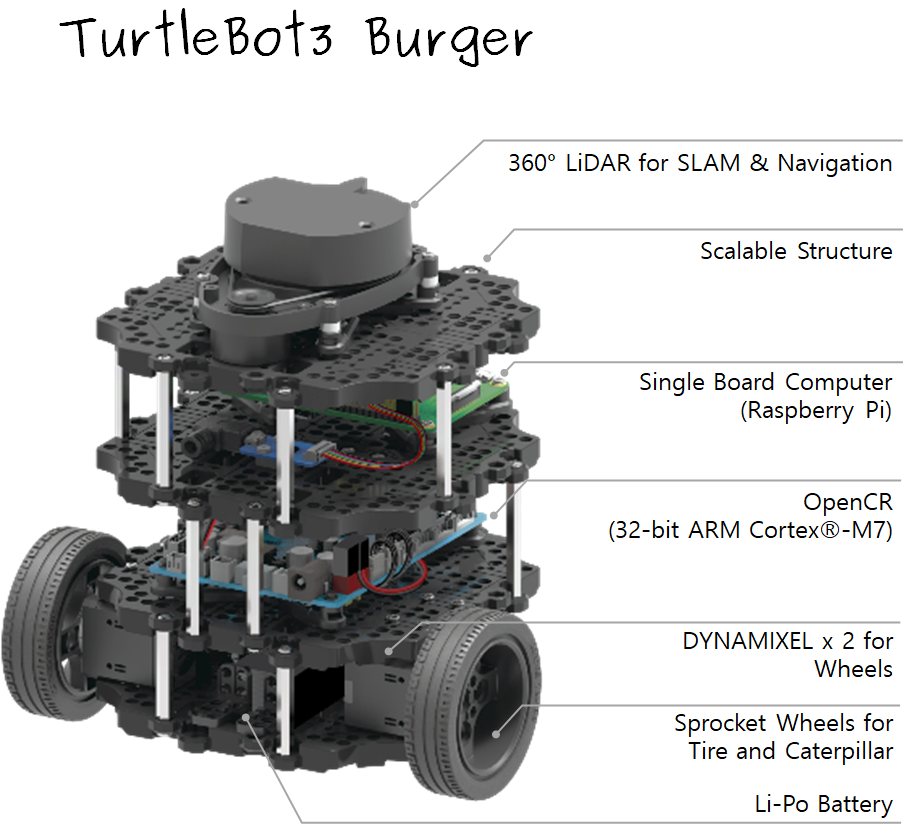
\includegraphics[width=10cm, height=8cm]{tb3-components.png}
\caption{scheda componenti del Turtlebot3 modello Burger}
\label{burger}
\end{figure}


\section{Risultati}

Nell'ultima sezione del capitolo saranno analizzati i risultati delle simulazioni effettuate con Gazebo. Nelle figure \ref{esempio} vengono riprodotti in sequenza i 4 frame di un tragitto compiuto dal robot verso la posizione target.

\begin{figure}[!htb]
    \centering
    \begin{minipage}{0.5\textwidth}
        \centering
        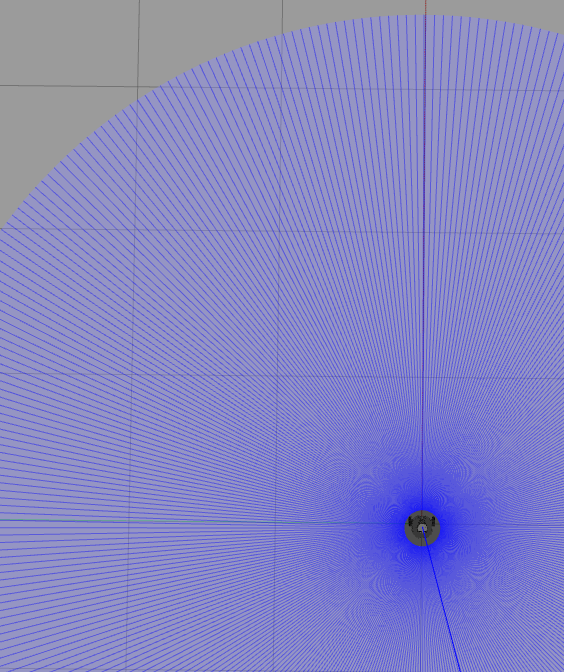
\includegraphics[width=0.8\textwidth, height=0.3\textheight]{frame1.png}
        \label{fig:prob1_6_2}
    \end{minipage}%
    \begin{minipage}{0.5\textwidth}
        \centering
        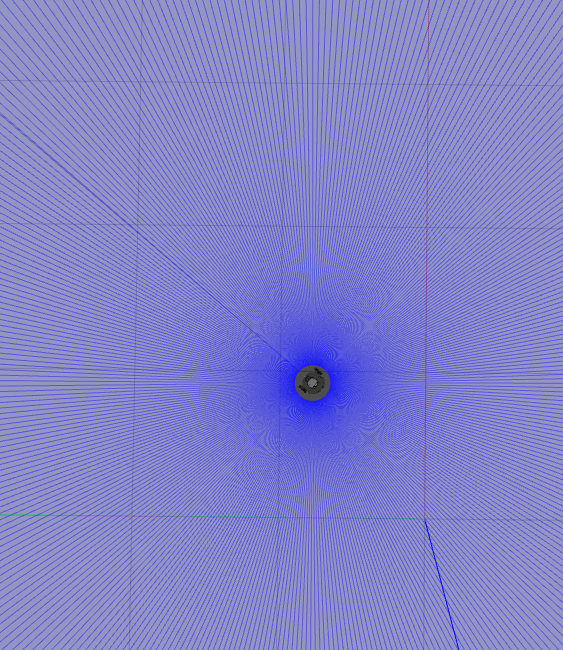
\includegraphics[width=0.8\textwidth, height=0.3\textheight]{frame2.png}
        \label{fig:prob1_6_1}
    \end{minipage}
\end{figure}
\begin{figure}[!htb]
    \centering
    \begin{minipage}{0.5\textwidth}
        \centering
        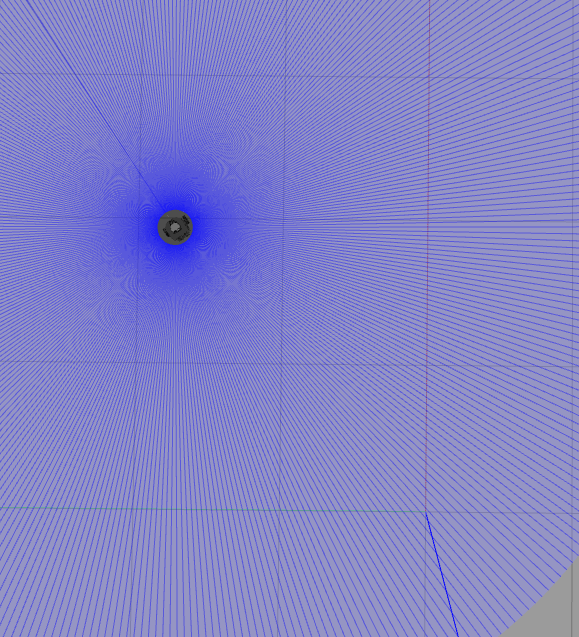
\includegraphics[width=0.8\textwidth, height=0.3\textheight]{frame3.png}
        \label{fig:prob1_6_2}
    \end{minipage}%
    \begin{minipage}{0.5\textwidth}
        \centering
        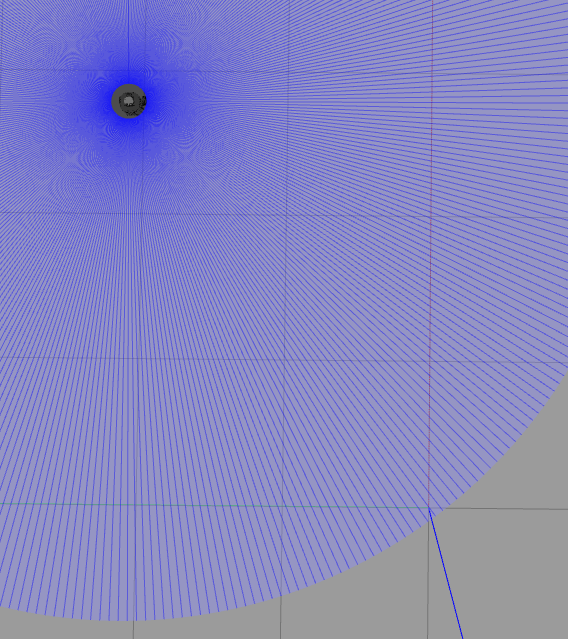
\includegraphics[width=0.8\textwidth, height=0.3\textheight]{frame4.png}
        \label{fig:prob1_6_1}
    \end{minipage}
    \label{esempio}
    \caption{Esempio di simulazione con Gazebo}
\end{figure}
\vspace{6cm}
Per verificare la correttezza della traiettoria saranno riportati e spiegati dei plot Matlab rappresentanti la posizione iniziale e finale del robot, selezionando un insieme di punti casuali.
Successivamente riproveremo gli stessi percorsi variando il valore $k_2$ di \eqref{cont-law}, fornendo adeguati commenti riguardo alla precisione e al cambiamento della forma della curva in base al cambiamento dei due valori.
Nella prima immagine, il pianificatore ha selezionato una manciata di punti casuali per testare l'affidabilità dell'architeturra e della legge di controllo. 
I punti selezionati sono $\emph{(3.0,2.0,0.52)}$, $ \emph{(3.0,1.0,0.14)}$, $\emph{(-3.0,-2.0,-0.15)}$  e $\emph{(3.0,1.0,0.52)}$. In particolare le traiettorie hanno come valori delle variabili $k_1=1$ e $ k_2=3$.
\\
Ecco il plot disegnati con Matlab delle varie posizione:

\begin{figure}[!htbp]
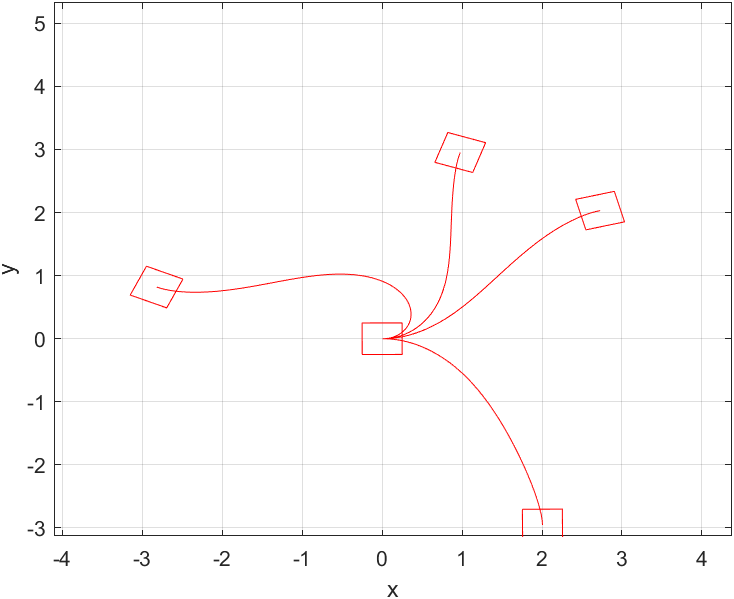
\includegraphics[width=10cm, height=10cm]{pos2.png}
\centering
\caption{Esempi dimostrativi di traiettorie di diversi punti nello spazio}
\label{burger}
\end{figure}
\vspace{7cm}
Infine imponiamo come target al robot $\emph{(3.0,2.0,0.58)}$ e vediamo le modifiche subite dalla traiettoria al variare di $k_2$. I valori testati sono $k_2=3$, $k_2=5$, $k_2=10$.
\begin{figure}[!h]
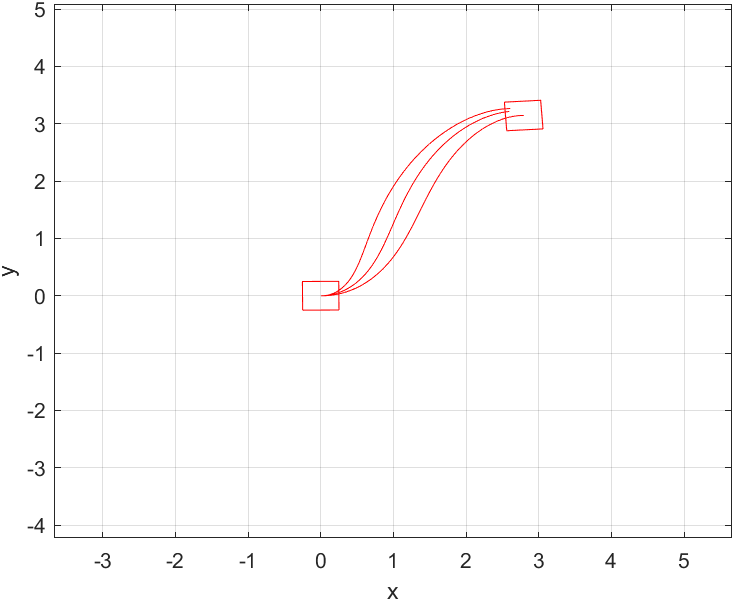
\includegraphics[width=10cm, height=10cm]{pos1.png}
\centering
\caption{Le diverse traiettorie al variare di $k_2$. Da $k_2=3$ in quella più bassa a destra a$k_2=10$ }
\label{burger}
\end{figure}


Dalle immagini qui sopra si può notare come il cambiamento di $k_2$ modifichi in maniera piuttosto accentuata la forma della traiettoria verso un determinato punto. All'aumentare di $k_2$ le curve diventano sempre più strette e quindi la convergenza alla traiettoria finale desiderata è molto più veloce e performante rispetto a dei valori bassi di $k_2$. Se infatti viene considerata la formula (2.1) è immediato notare che il termine $k_2$ elevato porta ad un maggiore aumento della velocità angolare che conseguentemente annulla lo sterzo e porta la stessa velocità angolare a valori molto bassi. In termini di una traiettoria questo si traudce con un repentino spostamento verso la posizione desiderata con un notevole appiattimento della curva percorsa.
In definitiva il controllore implementato nell'elaborato garantisce un'elevata elasticità rispetto a molteplici situazioni, dalla traiettoria più morbida ma sicura con $k_2$ basso, ad una traiettoria più decisa con un valore di $k_2$ molto alto. 


\chapter{Conclusioni}
Il controllore implementato permette la navigazione di robot mobili terrestri con un alto grado di fiducia e di efficienza attraverso una piattaforma open-source, che sempre di più negli ultimi anni ha guadagnato popolarità e fiducia nella comunità di sviluppatori in ambito di robotica. Inoltre la struttura molto modulare dell'applicazione consente future estensioni di ciascun componente. Il pianificatore potrebbe essere di fatto esteso in numerosi modi che andrebbero ad arricchire particolarmente la sua complessità ed efficacia tramite algoritmi sempre più evoluti e influenzate da altre discipline come il machine-learning o la computer vision. Invece nel caso del controllore, il primo passo da svolgere sarebbe quello di implementare il meccanismo delle actions di ROS 2 per ottenere una maggiore consapevolezza del tragitto percorso e un meccanismo di feedback più corpulento. Ma successivamente sarebbe possibile decidere di cambiare il robot utilizzato o la legge di controllo senza particolari modifiche nel codice evitand eccessivi costi in termini di tempo e  altrettante risorse.

	%\bibliographystyle{elsarticle-num}
	\bibliography{bibliografia}
	\bibliographystyle{IEEEtran}

\end{document}